\documentclass[10pt,a4paper]{article}
\usepackage[hyperref]{acl2019}
\usepackage{times}
\usepackage{latexsym}
\usepackage{graphicx}

\usepackage{url}

\aclfinalcopy % Uncomment this line for the final submission
%\def\aclpaperid{***} %  Enter the acl Paper ID here

%\setlength\titlebox{5cm}
% You can expand the titlebox if you need extra space
% to show all the authors. Please do not make the titlebox
% smaller than 5cm (the original size); we will check this
% in the camera-ready version and ask you to change it back.

\newcommand\BibTeX{B\textsc{ib}\TeX}

\title{Parallel Programming CSCI 4320 Project Report: \\
City Traffic Discrete Event Simulation}
\author{Alex Garten \\
  RPI \\
  \texttt{gartea@rpi.edu} \\\And
  Shoshana Malfatto \\
  RPI \\
  \texttt{malfas@rpi.edu} \\}

\date{}

\begin{document}
\maketitle
\begin{abstract}
    We implemented a parallel discrete event simulator for traffic patterns at intersections using C and MPI.
\end{abstract}

\section{Introduction}

Our goal was to implement a parallel discrete event simulator which models vehicle traffic patterns to reveal which traffic rules result in the shortest trips between a location A and location B, in a large grid modeled after a city. Though implementations of traffic pattern DES already exist, we will use this as an opportunity to learn how to create a DES, since they have many applications.

\section{Background}
Our knowledge of parallel discrete event simulators (PDES) comes originally from the course lecture. Parallel DES help represent large-scale systems that are hard to understand, and which may require long run times if represented in real-time. A parallel DES should significantly reduce the run time. For instance, a simulation of air traffic could take a few minutes instead of a several years by looking at only specific events that are deemed important, and looking at them in parallel when possible. This could be applied to many other topics like communication networks or biology.\\
\tab In class we talked about Rensselaer’s Optimistic Simulation System (ROSS) which runs Time Warp, a protocol that increases parallelism through rollback and anti-message mechanisms. This protocol scales very well in performance tests on RPI's Blue Gene/Q. We could have chosen to use ROSS to build our implementation, but we decided to create our simulator from scratch.

\section{Implementation}

We started with an implementation with a more complex grid, but started having memory errors close to the deadline which we would have struggled to find in time for submission, so we went with a simpler grid for our second implementation. However, we will go over the initial implementation since that was our idea going into this project and we spent time writing it, and because we kept many of the plans for this first implementation were maintained in the second implementation.

\subsection{Initial Implementation}

We used a conservative approach to build our parallel DES, where cars can stop at a discrete number of locations, and at most one movement could occur within a tick. In our large city, which was a grid of streets going either north-south or east-west, cars only needed to know about the cars near them, so traffic could run somewhat independently in different regions. However, synchronization is required to accurately move cars across the borders of their region.

For parallelization we used MPI, which we preferred to relying on threads after seeing the performance of both in Assignment 4/5. We used a side length for our grid of 32,768 blocks. For the full number of rows, this was multiplied by 2 so that even rows correspond to global coordinates of east-west streets, and odd rows correspond to global coordinates of north-south streets. The rows get divided up by the number of ranks, so that there would need to be communication with "ghost rows" like in homework 4/5.

\begin{figure}
    \centering
    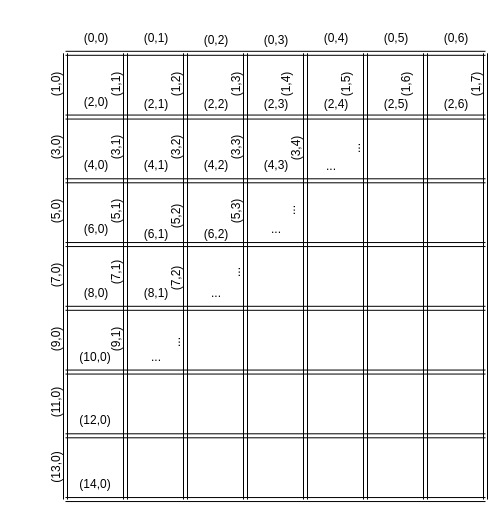
\includegraphics[scale=0.4]{parallel.jpg}
    \caption{Original street design, with SIDE\_LENGTH = 8, and therefore SIDE\_LENGTH*SIDE\_LENGTH intersections and 2*(SIDE\_LENGTH-1)*(SIDE\_LENGTH-1) streets (where you consider a street as just one block). The global index is displayed for some of the streets. Even row indices correspond to horizontal streets, and odd row indices correspond to vertical streets.}
    \label{fig:my_label}
\end{figure}

Each street was a C struct that contained an array for the lane going in one direction (east or south) and the lane going in the opposite direction (west or north). Each lane could hold 4 cars at one time. This resembled a queue, which is a commonly seen data structure in discrete event simulators.

There are intersection structs for each place where four streets should meet. This made moving cars cleaner for the programmer to implement and read.

\begin{figure}
    \centering
    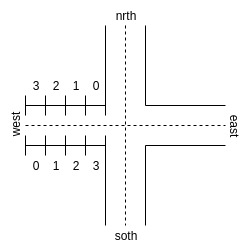
\includegraphics[scale=0.6]{parallel2.jpg}
    \caption{An intersection, including street indices from initial implementation (when each lane on a block had four locations). There can be at most 4 cars going through an intersection at a time.}
    \label{fig:my_label}
\end{figure}

The beginning of the simulation started with cars being randomly generated at locations on the grid, with random destinations. These locations are represented by a row index, a column index, and a street index which corresponds the eastern or southern direction.

At each step in time, or 'tick', ghost rows were sent between ranks. This required sending arrays of car objects, which are not an MPI\_Datatype.

Then intersections were updated according to the specified rules. Cars tried to turn in a direction that would get them closer to their destination on the global grid, but they must follow the rules of the road and not crash into other cars. For instance, if the car at the northern side of the intersection goes straight south, the car on the eastern side of the intersection can't go any direction but right within that tick of time. Then the streets would be updated by moving cars along them. Each car was supposed to move at most one grid location per tick.

Our program worked with only 1 rank, but when multiple ranks were used, the program would terminate unexpectedly. There were so many places that memory could be used incorrectly, and parallel programs are difficult to debug, so after some time spent trying to discover the bug, we changed plans to a different implementation of the city traffic problem.

\subsection{Final Implementation}

We kept many of the same details from the initial implementation, but now there are only intersections and no streets. Intersections are where complicated right-of-way rules can show up, so reducing the traffic problem to intersections is still useful, and should result in a more efficient simulation. This also means we do not have to create street arrays, which needed a strange indexing system because of the combination of horizontal (east-west) and vertical (north-south) rows.

Using only intersection structs and leaving no space on the street (which was used like a queue or buffer) makes synchronization more difficult because ranks on border a region which is controlled by a single rank must communicate regularly to find out if a car is coming along that intersection

\section{Performance Results}

\section{Analysis of Performance}

\section{Conclusion}

\bibliography{acl2019}
\bibliographystyle{acl_natbib}


\end{document}
